\section{Introduction}
% Why should we care?
Transformer-based large language models underpin a wide range of modern AI systems, from conversational agents to code generation and scientific reasoning. As these models continue to scale, practical deployment is increasingly constrained by inference cost, encompassing both computation and memory. As a result, a central objective in modern model design is to maximize achievable accuracy under fixed inference cost constraints.

% What is the problem?
Mixture-of-Experts (MoE) architectures have emerged as a promising approach towards this goal, enabling models to scale parameter count while keeping the number of Floating-point Operations (FLOPs) per token fixed. Despite their empirical success, the MoE design space remains poorly understood. Existing MoE architectures are largely motivated by high-level sparsity arguments and are optimized primarily for offline, throughput-oriented settings, with limited consideration of online deployments that impose strict latency, memory bandwidth, and communication constraints.

We argue that effective MoE design must be evaluated along two complementary dimensions: accuracy per FLOP and accuracy per parameter. While accuracy per FLOP captures computational efficiency, accuracy per parameter reflects memory footprint, memory bandwidth demands, routing-induced communication, and sharding overheads (factors that are often the dominant bottlenecks in interactive, low-latency inference). Neglecting these factors can lead to architectures that appear efficient in aggregate compute, yet incur substantial inefficiencies in practical deployment.

% How are we solving it?

\begin{figure}[h!tb]
    \centering
    \begin{subfigure}[b]{0.42\textwidth}
        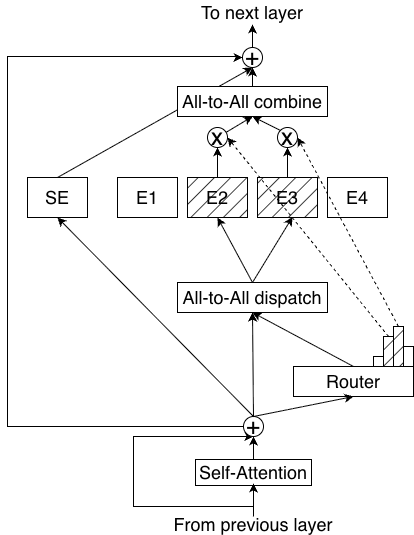
\includegraphics[width=\textwidth]{figures/standard_moe.png}
        \caption{Standard MoE architecture.}
        \label{fig:standard_moe}
    \end{subfigure}
    \hfill
    \begin{subfigure}[b]{0.45\textwidth}
        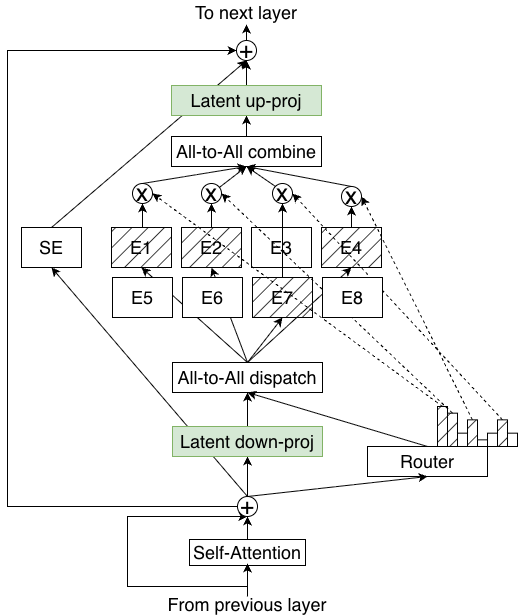
\includegraphics[width=\textwidth]{figures/latent_moe.png}
        \caption{LatentMoE architecture.}
        \label{fig:latent_moe}
    \end{subfigure}
    \caption{Standard MoE vs. LatentMoE architectures. In LatentMoE, tokens are projected from the model hidden dimension $d$ into a smaller latent dimension $\ell$ for expert routing and computation, which reduces routed parameter loads and all‑to‑all traffic by a factor of $d / \ell$. We use this efficiency to increase the total number of experts and the top-k active experts per token by the same factor $d/\ell$, which improves the accuracy of the model while keeping overall inference cost approximately constant.}
    \label{fig:intro_fig}
\end{figure}

In this work, we revisit MoE architecture design from a hardware–software co-design perspective. Through a systematic analysis of existing MoE systems across the throughput–latency Pareto frontier, we identify key structural bottlenecks arising from expert parameterization, routing-induced all-to-all communication, and memory access patterns. Combined with detailed accuracy measurements and theoretical analysis, our study identifies structural inefficiencies in prevailing MoE designs that limit achievable accuracy per unit of inference cost.


Guided by these insights, we introduce LatentMoE, a new mixture-of-experts architecture explicitly optimized for both accuracy per FLOP and accuracy per parameter. LatentMoE decouples expert routing and computation from the model hidden dimension by projecting incoming activations into a shared low-dimensional latent space prior to expert processing (Figure~\ref{fig:intro_fig}). The latent dimension serves as a direct control knob for computational cost, communication volume, and expert parameter size. At iso-FLOP and iso-parameter count, projecting incoming activations into a lower-dimensional latent space enables a proportional increase in both the number of experts and the routing top-k, while maintaining constant inference cost. 

As we show both theoretically and empirically, simultaneously increasing expert count and combinatorial sparsity diversity improves the effective expressivity of the model, leading to higher achievable accuracy. Crucially, these gains arise without increasing memory bandwidth demands or communication overheads, making LatentMoE well suited for both latency-critical and throughput-oriented deployments. We validate the LatentMoE concept through pretraining experiments at scales of up to 95B parameters and over 1T tokens. Across all evaluated regimes, LatentMoE consistently improves upon standard MoE architectures, achieving higher accuracy at fixed inference cost or substantially lower inference cost at fixed accuracy. Given its strong performance, the LatentMoE architecture has been adopted by the flagship Nemotron-3 Super and Ultra models and scaled to substantially larger regimes, including longer token horizons and larger model sizes~\citep{nvidia2025nvidianemotron3efficient}.
